\documentclass[11pt]{article}
\usepackage{enumerate}
\usepackage{fancyhdr}
\usepackage{amsmath}
\usepackage{graphicx}

\thispagestyle{empty}
\setlength{\parindent}{0cm}
\setlength{\parskip}{0.3cm plus4mm minus3mm}
\oddsidemargin = 0.0in
\textwidth = 6.5 in
\textheight = 9 in
\headsep = 0in

\title{CSCI 4100 Fall 2018 \\
% enter assignment number
Assignment 6 Answers}
\author{Damin Xu\\661679187}

\begin{document}
\maketitle
% enter question #
\noindent{\bf Exercise 3.4}
\begin{enumerate} [(a)]
	\item From the question, $\epsilon = [\epsilon_1,\epsilon_2,...,\epsilon_N]^T$, $y = [y_1,y_2,...,y_N]$, $X = [x_1,x_2,...,x_3]$, so, $y = X\omega^*+\epsilon$.\\

	Because $w_{lin}=((X^TX)^{-1}X^T)y$ and $H=X(X^TX)^{-1}X^T$, \\so $\hat{y}=Xw_{lin}=X(X^TX)^{-1}X^Ty=Hy=H(X\omega^*+\epsilon)=X(X^TX)^{-1}X^TX+H\epsilon=1X\omega^*+H\epsilon\\=X\omega^*+H\epsilon$

	\item Since $\hat{y}=X+H\epsilon$,
	\\$\hat{y}=X\omega^*+H\epsilon-y = X\omega^*+H\epsilon-(X\omega^*+\epsilon)\\=\epsilon(H-I)$

	\item \[
		\begin{aligned}
		E_{in}(w)&=\frac{1}{N}||Xw-y||^2\\
		&= \frac{1}{N}||Xw^*+H\epsilon-y||^2\\
		&= \frac{1}{N}||\hat{y}-y||^2\\
		&= \frac{1}{N}||(H-I)\epsilon||^2\\
		&= \frac{1}{N}((H-I)\epsilon)^T((H-I)\epsilon)\\
		&= \frac{1}{N}\epsilon^T(H-I)^2\epsilon\\
		&= \frac{1}{N}\epsilon^T(I-H)^2\epsilon\\
		\end{aligned}
	\]
	From exercise(c),$ (I-H)^K=I$ for any K,\\
	So, \[
		E_{in}(w)=\frac{1}{N}\epsilon^T(I-H)\epsilon\\
	\]
	\newpage
	\item because $trace(H) = d+1$, \[ 
		\begin{aligned}
		E_D[E_{in}(w)] &= \frac{1}{N}E_D(\epsilon^T(I-H)^2\epsilon)\\
		&= \frac{1}{N}E_Dtrace(\epsilon^T(I-H)^2\epsilon)\\
		&= \frac{1}{N}(N\sigma^2-(\sum^N_{i=1}H_{ii})\sigma^2)
		&= \frac{1}{N}(N\sigma^2-trace(H)\sigma^2)\\
		&= \frac{1}{N}(N\sigma^2-(d+1)\sigma^2)\\
		&= \sigma^2(1-\frac{d+1}{N})
		\end{aligned}
	\]
	\item First from part (a), $\hat{y} = X\omega^*+\epsilon$,\\
	So, \[
		\begin{aligned}
		E_{test}(w_{lin})=\frac{1}{N}||\hat{y}-y'||^2\\
		&= \frac{1}{N}(\epsilon^TH-\epsilon'^{T}(H\epsilon-\epsilon'))\\
		&= \frac{1}{N}(\epsilon^THH\epsilon-2\epsilon'^TH\epsilon+\epsilon'^T\epsilon')\\
		&=\frac{1}{N}(\epsilon^TH\epsilon-2\epsilon'^TH\epsilon+\epsilon'^T\epsilon')
		\end{aligned}
	\]
	Then $E_{D,\epsilon'}[E_{in}(w_{lin})]=E_{D,\epsilon'}[\frac{1}{N}(\epsilon^TH\epsilon-2\epsilon'^TH\epsilon+\epsilon'^T\epsilon')]$\\
	From part (d), $E_D(\epsilon^T\epsilon)=N\sigma^2$ and $E_D(\epsilon^TH\epsilon)=(d+1)\sigma^2$,\\\\
	So, $E_{D\epsilon'}[E_{in}(w_{lin})]=\sigma^2(1+\frac{d+1}{N})-\frac{2}{N}E_{D,\epsilon'}(\epsilon'^TH\epsilon)]$\\\\
	\\Because $E_{D,\epsilon'}(\epsilon'^TH\epsilon)=\sum^N_{i=1}(E(\epsilon'_i)H_{ii}E(\epsilon_i))=0$, \[
		E_{D\epsilon'}[E_{in}(w_{lin})] = \sigma^2(1+\frac{d+1}{N})
	\]
\end{enumerate}
\newpage

\noindent{\bf Problem 3.1}
\begin{enumerate} [(a)]
	\item \ \\
	\begin{figure}[htb]
		{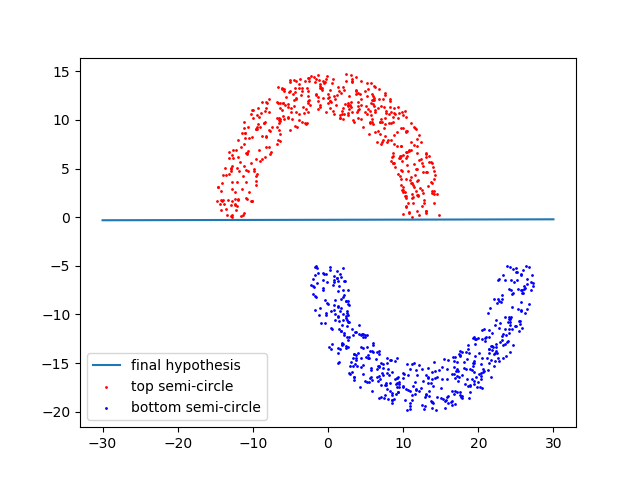
\includegraphics[height=7cm]{p3_1_a.png}}
	\end{figure}
	\item \ \\
	\begin{figure}[htb]
		{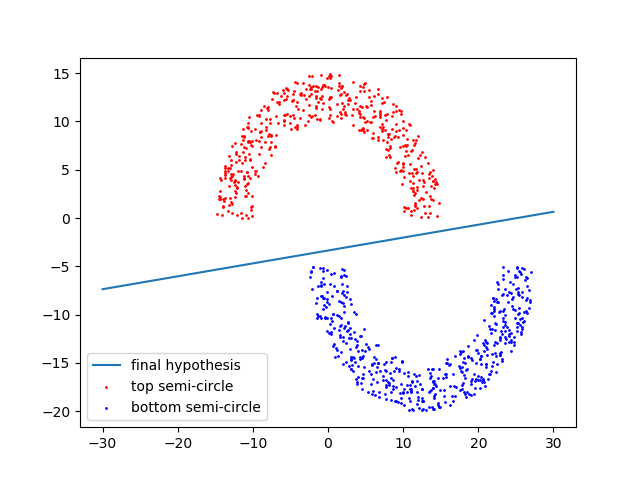
\includegraphics[height=7cm]{p3_1_b.png}}
	\end{figure}

	By linear regression, the final hypothesis is much more colse to the center of two semi-circles then by PLA, because linear regression consider y as real number instead of a sign, which makes result more precise.
\end{enumerate}

\newpage

\noindent{\bf Problem 3.2}\\
\begin{figure}[htb]
	{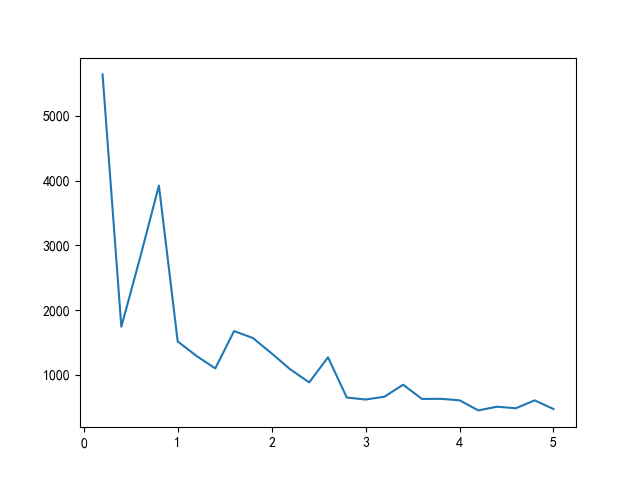
\includegraphics[height=7cm]{p3_2.png}}
\end{figure}\\
As the graph showed, the number of iterations decreases as the $sep$ increase.\\
From Problem 1.3, we know that\[
	t \leq \frac{R^2||w^*||^2}{\rho^2}
\] Here because two semi-circles are fixed, so $R$ is a constant.\\
Then As $sep$ increases, the shortest distance between two points gets larger, which makes $\frac{||w^*||}{\rho}$ smaller. Hence $t$ gets smaller, and the number of iteration is getting smaller.

\newpage

\noindent{\bf Problem 3.8}
\begin{enumerate} [(1)]
	\item Show that among all hypotheses. the one that minimizes $E_{out}$ is given by $h^*(x)=E[y|x]$:
	\[
		\begin{aligned}
			E_{out}(h)&=E[(h(x)-y)^2]\\
			&=E[((h(x)-h^*(x))+(h^*(x)-y))^2]\\
			&=E[(h(x)-h^*(x))^2]+E[(h^*(x)-y)^2]+2E[(h(x)-h^*(x))(h^*(x)-y)]
		\end{aligned}
	\]
	Hence, to minimize $E_{out}$, we need minimize $2E[(h(x)-h^*(x))(h^*(x)-y)]$.\\
	Let $h^*(x)=E[y|x]$:\[
		\begin{aligned}
			E[(h(x)-h^*(x))(h^*(x)-y)] = E[(h(x)-h^*(x))(h^*(x)-y)]\\
			&=E[(h(x)-h^*(x))(h^*(x)-h^*(x))]\\
			&=0
		\end{aligned}
	\]
	Therefore, when $h^*(x)=E[y|x]$, $E_{out}$ is minimized.

	\item Becasue $E(E(y|x))=E(y)$, 
	\\$E[\epsilon(x)]$\\
	$=E[E[\epsilon(x)|x]]$\\
	$=E[E[y-h^*(x)|x]]$\\
	$=E[E[E(y|x)-E(h^*(x)|x)]]$\\
	$=E[h^*(x)-h^*(x)]$\\
	$=0$
\end{enumerate}
\newpage
\noindent{\bf Handwritten Digits Data - Obtaining Features}
\begin{enumerate} [(a)]
	\item This is plot for an 1 digit:\\
	\begin{figure}[htb]
		{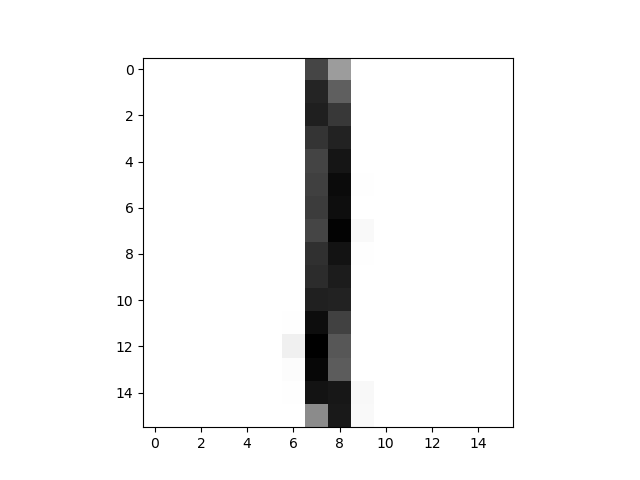
\includegraphics[height=7cm]{digit1.png}}
	\end{figure}\\
	This is plot for a 5 digit:\\
	\begin{figure}[htb]
		{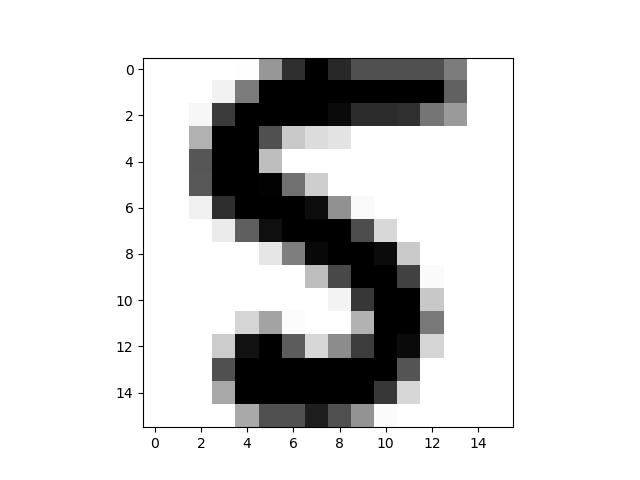
\includegraphics[height=7cm]{digit5.png}}
	\end{figure}

	\newpage

	\item Feature 1: Let $M$ be a matrix for a digit,\[
		intensity = \sum^{15}_{i=0}\sum^{15}_{j=0}M_{i,j}
	\]
	Feature 2: Let $M_{a,b}$ and $M_{c,d}$ be two position in a digit.\\
	Let $(M_{a,b} == M_{c,d}) = 1$ if $M_{a,b} = M_{c,d}$;\\
	Let $(M_{a,b} == M_{c,d}) = 0$ if $M_{a,b} != M_{c,d}$.\\
	So,\[
		symmetry = \sum^{16}_{i=0}\sum^7_{j=0}((M_{i,j} == M_{i,15-j})
	\]


	\item This is a plot of features for each digits:\\
	\begin{figure}[htb]
		{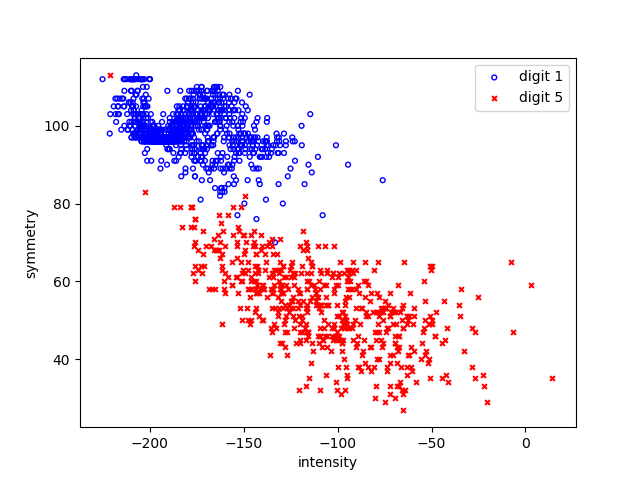
\includegraphics[height=10cm]{features.png}}
	\end{figure}
\end{enumerate}
\end{document}
\end{document}
